% <!-- coding: utf-8 -->
%
% la page de garde
% http://www.jujens.eu/posts/2013/Oct/20/latex-page-garde/
\begin{titlepage}
  \begin{sffamily}
  \begin{center}

    % Upper part of the page. The '~' is needed because \\
    % only works if a paragraph has started.


    \textsc{\LARGE Bretagne Vivante Rennes}\\[1cm]
    \textsc{\Large Vilaine Aval - oiseaux en hiver}\\[1cm]

    % Title
    \HRule \\[0.4cm]
    { \huge \bfseries \monsoustitre}
    \HRule \\[0.4cm]
    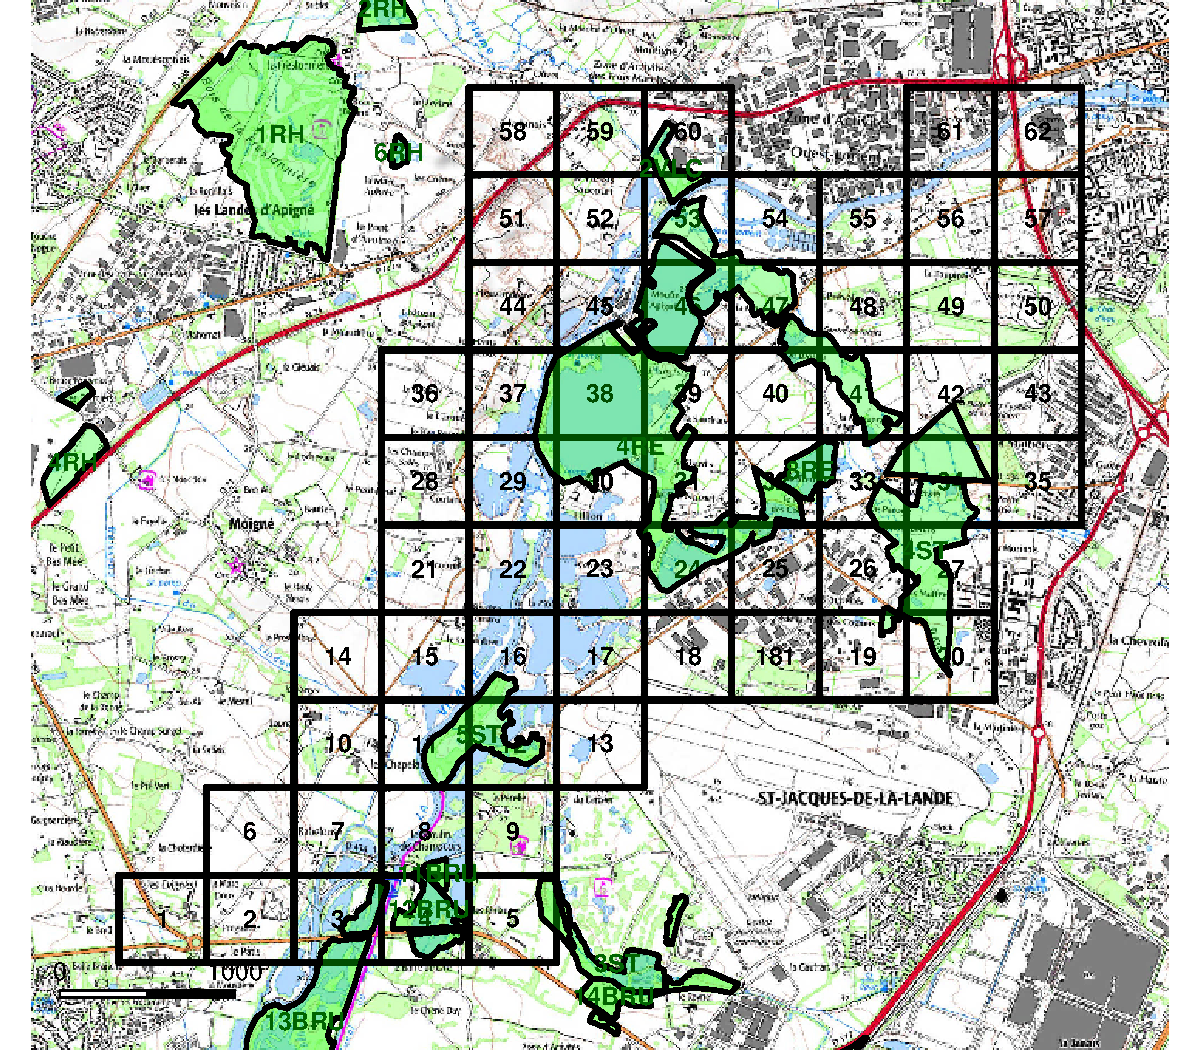
\includegraphics[width=190mm]{images/territoire_Nord.pdf}~\\[.5cm]
    \HRule \\[0.4cm]
    \begin{minipage}{0.4\textwidth}
      \begin{flushleft} \large
        \emph{Coordination}\\
        Matthieu Beaufils\\
         Marc Gauthier
      \end{flushleft}
    \end{minipage}
    \begin{minipage}{0.4\textwidth}
      \begin{flushright} \large
        \emph{Informatique}\\
        Marc Gauthier
      \end{flushright}
    \end{minipage}

    \vfill
  \end{center}
  \end{sffamily}
\end{titlepage}
